\documentclass[11pt]{amsbook}

\usepackage[turkish]{babel}
\usepackage{../Ceyhun}
\usepackage{../amsTurkish}

\begin{document}
\hPage{219}
Örneğin, \reffig{fig:ceyhun-219-Sekil4.4.2} deki Ç çizgesini düşünelim. Bu çizgeden d\textsubscript{0} düğümünün çıkarılması, düğümleri tek sayıya eşit 3 parça oluşturmaktadır. Bu sayı çıkarılan düğüm sayısından büyük olduğu için Ç(d,a) da 1-ayrık yoktur.
\begin{figure}[h]
	\centering
	\includegraphics[width=0.6\textwidth]{images/ceyhun-219-fig01}
	\caption{Teorem \ref{Teorem4.4.1} in açıklanması}
	% I do not know the exact label of the Teorem4.4.1 because it is in another page.
	\label{fig:ceyhun-219-Sekil4.4.2}
\end{figure}
\\Teorem \ref{Teorem4.4.1} i uygun biçimde ve yeterince uygulayarak bir çizgenin, eğer varsa 1-ayrışımı
% I do not know the exact label of the Teorem4.4.1 because it is in another page.
\end{document}